\section{Vérification de la correction}

Afin de vérifier si la correction appliquée est correcte, nous allons procéder en trois étapes.

\subsection{Tests du programme}

La première partie de vérification est celle de l'utilisation du programme. Il est en effet possible de tester le programme afin de voir si tous les cas imaginables par l'utilisateur sont pris en compte.

\subsection{Analyseur statique}

Un analyseur statique est un programme qui va analyser le code source d'un autre programme. Celui-ci va ainsi donner des conseils quand à l'utilisation de certaines fonctions au sein du code.\\
Ici, nous utiliserons l'analyseur statique \textit{FlawFinder}.\\
En l'utilisant sur le code de base, nous obtenons la sortie suivante :
\begin{figure}[H]
  \centering
  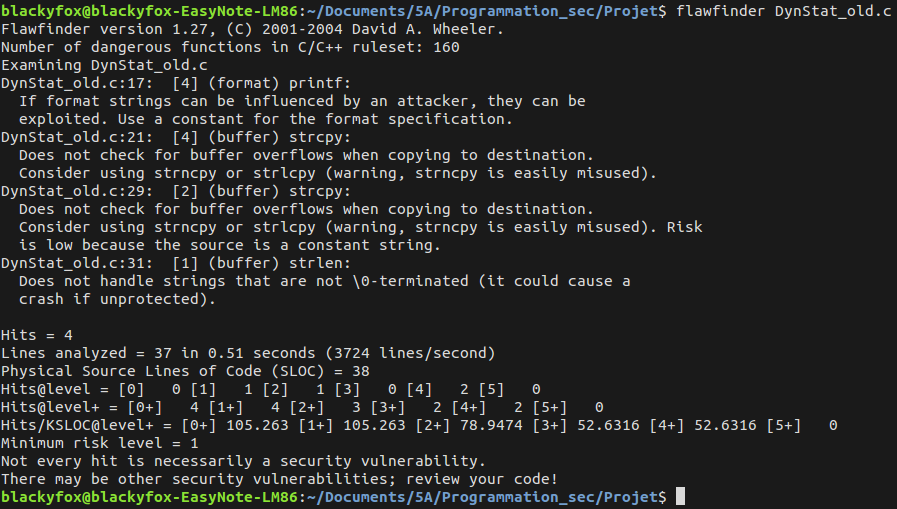
\includegraphics[width=.9\textwidth]{img/conc1.png}
  \caption{Résultat de \textit{FlawFinder} sur le code de base}
  \label{img:conc1}
\end{figure}
Comme nous pouvons le voir plusieurs fonctions sont à examiner de plus près d'après \textit{FlawFinder} :
\begin{enumerate}
 \item La fonction \textit{printf} ligne 17. Cette dernière prend en argument seulement \textit{argv[1]} ce qui peut permettre à des attaquants d'utiliser du code formaté pour détourner l'utilisation du programme.
 \item La fonction \textit{strcpy} lignes 21 et 29. Cette fonction ne vérifie pas si le buffer de destination est assez grand pour accueillir le contenu du buffer d'arrivé. Il y a alors un risque de \textit{buffer overflow}.
 \item La fonction \textit{strlen} ligne 31. Comme expliqué précédemment (c.f. \ref{buf22}), cette fonction ne gère pas le caractère de fin de chaîne et peut ainsi faire planter le programme en cas de mauvaise gestion.
\end{enumerate}
En utilisant \textit{FlawFinder} sur notre code corrigé, nous obtenons le résultat suivant :
\begin{figure}[H]
  \centering
  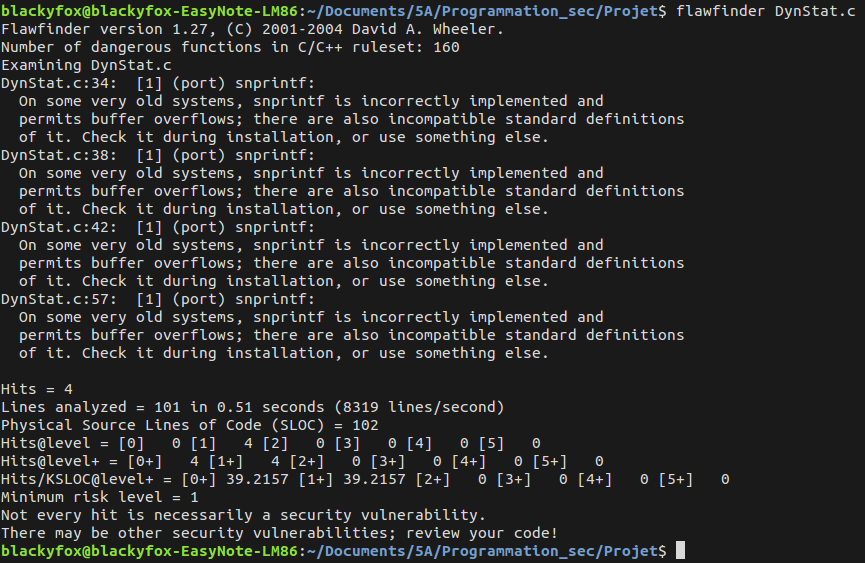
\includegraphics[width=.9\textwidth]{img/conc2.png}
  \caption{Résultat de \textit{FlawFinder} sur le code corrigé}
  \label{img:conc2}
\end{figure}
Ici, nous pouvons clairement voir qu'une seule fonction n'est remarquée par \textit{FlawFinder} : \textit{snprintf} lignes 34, 38, 42 et 57.\\
L'analyseur nous indique que dans de vieux systèmes cette fonction était mal implémentée et qu'il faut alors se prémunir de certains risques pour ce genre de systèmes. Dans notre cas, cela n'a que peu d'importance. En effet, en ayant utilisé des tests conditionnels autour des valeurs de retour de cette fonction, nous nous protégeons de potentielles erreurs.\\
Ainsi, nous pouvons dire que notre code corrigé est valide selon \textit{FlawFinder}.

\subsection{Analyseur dynamique}

Cependant, comme expliqué dans le point précédent, un analyseur statique ne s'occupe que du code source et non de l'exécution du programme. Ainsi, pour vérifier s'il n'y a pas de fuite mémoire dans notre code, nous utiliserons l'outil \textit{Valgrind}.\\
Nous allons pouvoir comparer les sorties de \textit{Valgrind} sur le programme d'origine et celui corrigé.
\begin{figure}[H]
  \begin{subfigure}[b]{0.45\textwidth}
    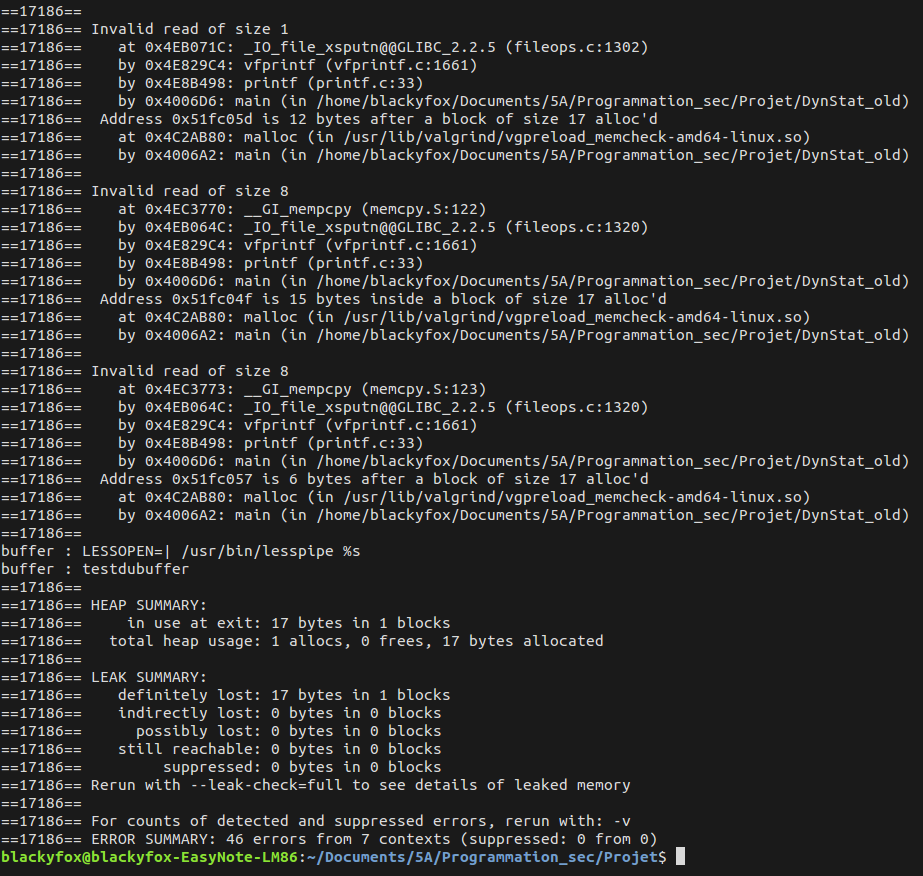
\includegraphics[width=\textwidth]{img/conc3.png}
    \caption{Résultat de \textit{Valgrind} pour le code original sans argument}
  \end{subfigure}
  ~
  \begin{subfigure}[b]{0.45\textwidth}
    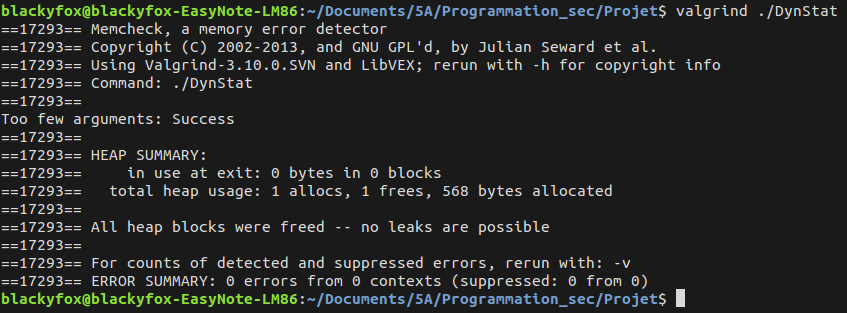
\includegraphics[width=\textwidth]{img/conc4.png}
    \caption{Résultat de \textit{Valgrind} pour le code corrigé sans argument}
  \end{subfigure}
  \caption{Résultat de \textit{Valgrind} pour une exécution sans argument}
\end{figure}

\begin{figure}[H]
  \begin{subfigure}[b]{0.45\textwidth}
    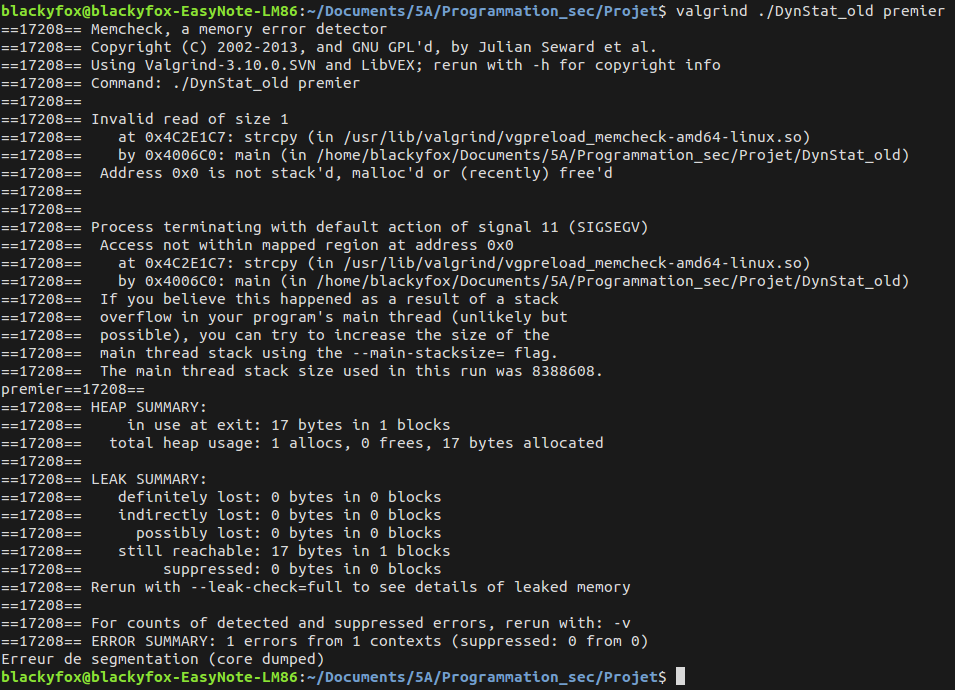
\includegraphics[width=\textwidth]{img/conc5.png}
    \caption{Résultat de \textit{Valgrind} pour le code original avec un argument}
  \end{subfigure}
  ~
  \begin{subfigure}[b]{0.45\textwidth}
    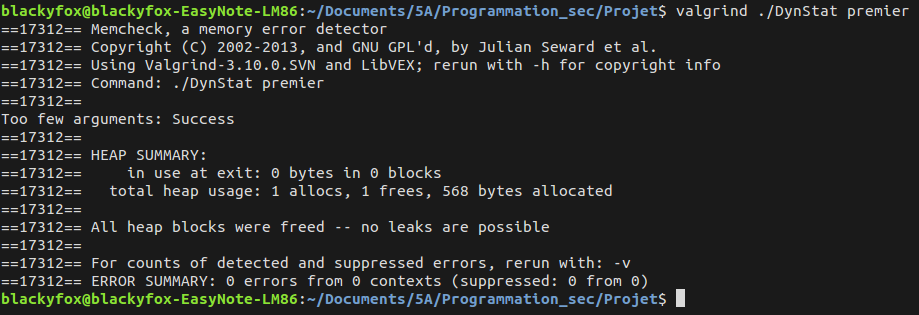
\includegraphics[width=\textwidth]{img/conc6.png}
    \caption{Résultat de \textit{Valgrind} pour le code corrigé avec un argument}
  \end{subfigure}
  \caption{Résultat de \textit{Valgrind} pour une exécution avec un argument}
\end{figure}

\begin{figure}[H]
  \begin{subfigure}[b]{0.45\textwidth}
    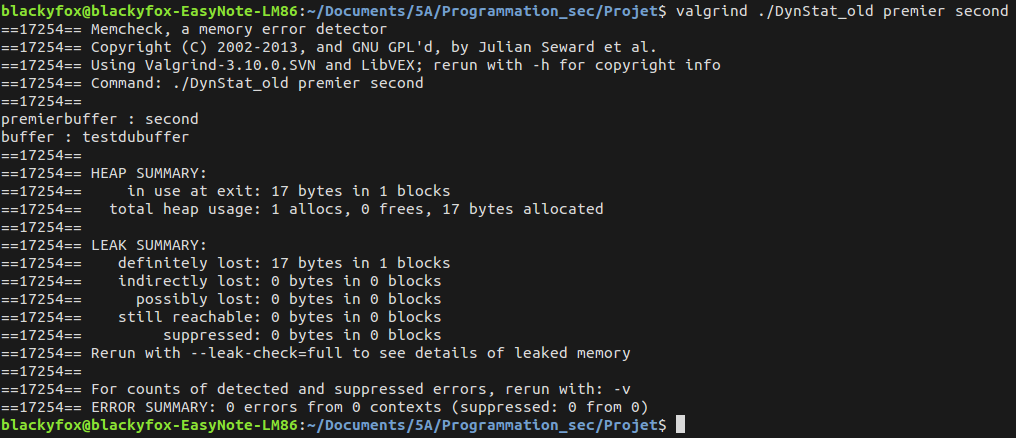
\includegraphics[width=\textwidth]{img/conc7.png}
    \caption{Résultat de \textit{Valgrind} pour le code original avec deux arguments}
  \end{subfigure}
  ~
  \begin{subfigure}[b]{0.45\textwidth}
    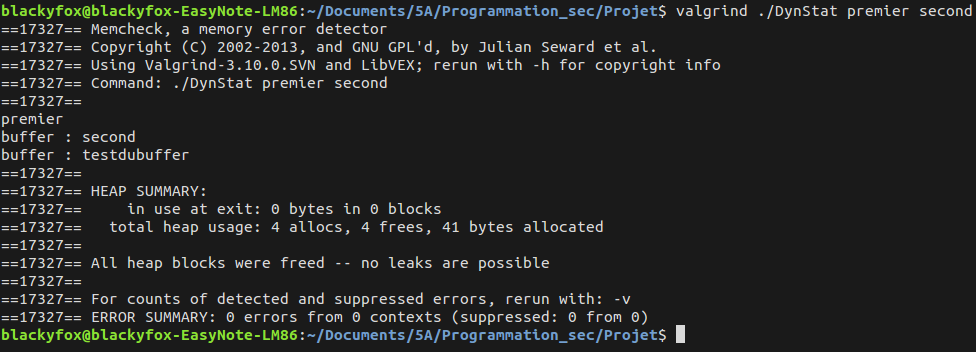
\includegraphics[width=\textwidth]{img/conc8.png}
    \caption{Résultat de \textit{Valgrind} pour le code corrigé avec deux arguments}
  \end{subfigure}
  \caption{Résultat de \textit{Valgrind} pour une exécution avec deux arguments}
\end{figure}

\begin{figure}[H]
  \begin{subfigure}[b]{0.45\textwidth}
    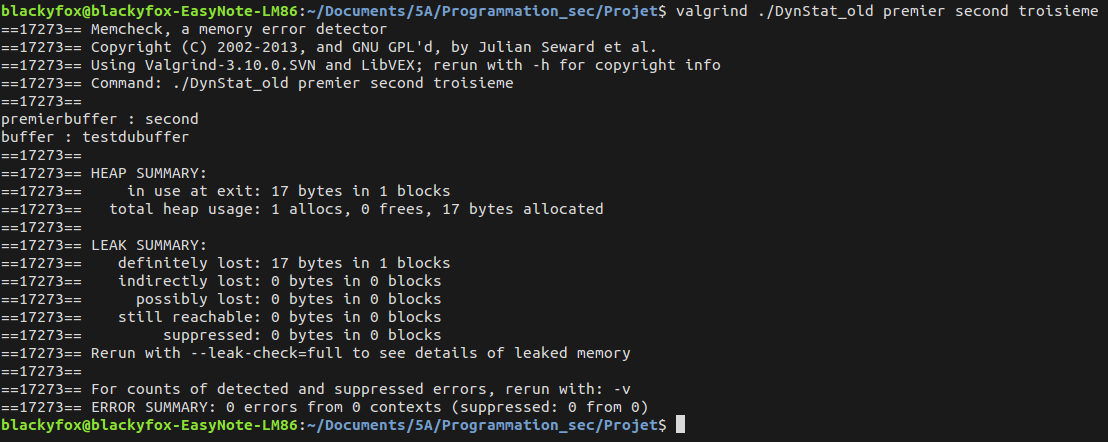
\includegraphics[width=\textwidth]{img/conc9.png}
    \caption{Résultat de \textit{Valgrind} pour le code original avec trois arguments}
  \end{subfigure}
  ~
  \begin{subfigure}[b]{0.45\textwidth}
    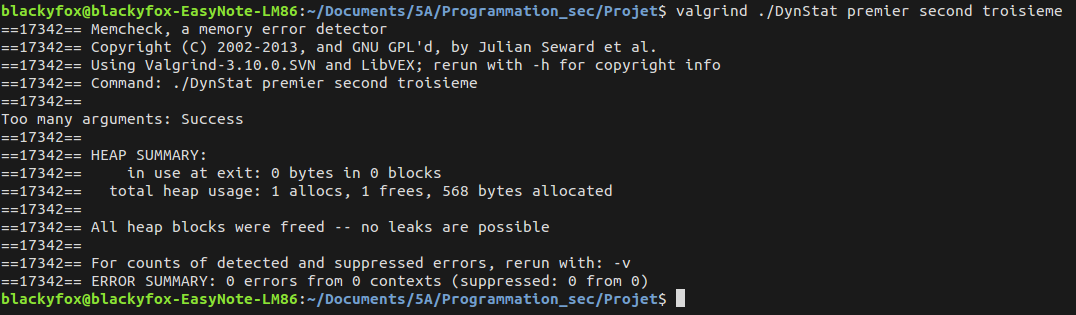
\includegraphics[width=\textwidth]{img/conc10.png}
    \caption{Résultat de \textit{Valgrind} pour le code corrigé avec trois arguments}
  \end{subfigure}
  \caption{Résultat de \textit{Valgrind} pour une exécution avec trois arguments}
\end{figure}
Comme nous pouvons le voir sur tous les screenshots ci-dessus, le code original à de nombreuses fuites mémoire (\textit{memory leak}) et des tentatives de lecture de zones mémoire protégées (\textit{Invalid read of size\ldots}).\\
Cependant, sur les screenshots de droite, ceux du code corrigé, nous pouvons remarquer que nous n'avons aucune fuite mémoire ni aucun accès à de la mémoire protégée.\\
Ainsi, nous pouvons conclure que ce code est sécurisée du point de vue de l'analyseur dynamique.